\documentclass[nooutcomes]{ximera}
%% handout
%% space
%% newpage
%% numbers
%% nooutcomes


\newcommand{\RR}{\mathbb R}
\renewcommand{\d}{\,d}
\newcommand{\dd}[2][]{\frac{d #1}{d #2}}
\renewcommand{\l}{\ell}
\newcommand{\ddx}{\frac{d}{dx}}
\newcommand{\dfn}{\textbf}
\newcommand{\eval}[1]{\bigg[ #1 \bigg]}

\usepackage{multicol}

\renewenvironment{freeResponse}{
\ifhandout\setbox0\vbox\bgroup\else
\begin{trivlist}\item[\hskip \labelsep\bfseries Solution:\hspace{2ex}]
\fi}
{\ifhandout\egroup\else
\end{trivlist}
\fi} %% we can turn off input when making a master document
\usepackage{fullpage}

\title{2.3:  Limit Laws}  

\begin{document}
\begin{abstract}		\end{abstract}
\maketitle


  The limits laws:
  
  Assume $\lim_{x \to a} f(x)$ and $\lim_{x \to a} g(x)$ both exist.
  The following properties hold, where $c$ is a real number and $m > 0$ and $n > 0$ are both integers.
  \begin{description}
      \item[Sum]
        \[
          \lim_{x \to a} \bigl(f(x) + g(x)\bigr) = \lim_{x \to a} f(x) + \lim_{x \to a} g(x)
        \]

      \item[Difference]
        \[
          \lim_{x \to a} \bigl(f(x) - g(x)\bigr) = \lim_{x \to a} f(x) - \lim_{x \to a} g(x)
        \]

      \item[Constant multiple]
        \[
          \lim_{x \to a} c \cdot \bigl( f(x) \bigr) = c \cdot \lim_{x \to a} f(x)
        \]

      \item[Product]
        \[
          \lim_{x \to a} \bigl(f(x) \cdot g(x)\bigr) = \bigl(\lim_{x \to a} f(x)\bigr) \cdot \bigl(\lim_{x \to a} g(x) \bigr)
        \]

      \item[Quotient]
        \[
          \lim_{x \to a} \left(\frac{f(x)}{g(x)}\right) = \frac{\lim_{x \to a} f(x)}{\lim_{x \to a} g(x)}, \text{provided} \lim_{x \to a} g(x) \ne 0
        \]   

      \item[ Power]
        \[
          \lim_{x \to a} \bigl(f(x)\bigr)^n = \bigl(\lim_{x \to a} f(x)\bigr)^n
        \]

      \item[Fractional power]
        \[
          \lim_{x \to a} \bigl(f(x)\bigr)^{n/m} = \bigl(\lim_{x \to a} f(x)\bigr)^{n/m},
        \]
        provided $f(x) \ge 0$, for $x$ near $a$, if $m$ is even and $n/m$ is reduced to lowest terms
    \end{description}

%Problem 1
\begin{problem}

  The following argument shows 
  \[
    \lim_{x \to 3} \frac{5x^3 - 4 \sqrt{x}}{\sqrt{x^5 - 87}} = \frac{135 - 4\sqrt{3}}{\sqrt{156}}.
  \]
  State which limit law is used to justify each step.
  (A particular step may have more than one limit law as a justification.)

  \begin{align*}
    \lim_{x \to 3} \frac{5x^3 - 4 \sqrt{x}}{\sqrt{x^5 - 87}}
    &= \frac{\lim_{x \to 3} 5x^3 - 4 \sqrt{x}}{\lim_{x \to 3}\sqrt{x^5 - 87}}\\
    &= \frac{5\lim_{x \to 3}(x^3) - 4 \lim_{x \to 3}\sqrt{x}}{\sqrt{\lim_{x \to 3}(x^5 - 87)}}\\
    &= \frac{5(\lim_{x \to 3}x)^3 - 4 \sqrt{3}}{\sqrt{\lim_{x \to 3}(x^5) - \lim_{x \to 3} (87)}}\\
    &= \frac{5(3)^3 - 4 \sqrt{3}}{\sqrt{3^5 - 87}}\\
    &= \frac{135 - 4\sqrt{3}}{\sqrt{156}}
  \end{align*}
  \begin{freeResponse}
    \begin{align*}
      \lim_{x \to 3} \frac{5x^3 - 4 \sqrt{x}}{\sqrt{x^5 - 87}}
      &= \frac{\lim_{x \to 3} 5x^3 - 4 \sqrt{x}}{\lim_{x \to 3}\sqrt{x^5 - 87}} \hspace*{5em}\parbox[b][]{3in}{(Quotient Limit Law)} \\
      &= \frac{5\lim_{x \to 3}(x^3) - 4 \lim_{x \to 3}\sqrt{x}}{\sqrt{\lim_{x \to 3}(x^5 - 87)}} \hspace*{3em}\parbox[b][]{3in}{(Difference, Constant Multiple, and Fractional Power Limit Laws)}\\
      &= \frac{5(\lim_{x \to 3}x)^3 - 4 \sqrt{3}}{\sqrt{\lim_{x \to 3}(x^5) - \lim_{x \to 3} (87)}} \hspace*{3em}\parbox[b][]{3in}{(Power and Difference Limit Laws)}\\
      &= \frac{5(3)^3 - 4 \sqrt{3}}{\sqrt{3^5 - 87}} \hspace*{5em}\parbox[b][]{3in}{(Power Limit Law)}\\
      &= \frac{135 - 4\sqrt{3}}{\sqrt{156}}
    \end{align*}
  \end{freeResponse}



\end{problem}


%problem 2
\begin{problem}
State the form of the limit and then evaluate the limit algebraically using the limit laws. 
	
	\begin{enumerate}
	
	%part a		
	\item $ \lim_{x \to 6} \frac{4x^2 - 144}{x-6}  $
	\begin{freeResponse}
	\begin{align*}
	\text{Form:} \frac{0}{0}\\
	\lim_{x \to 6} \frac{4x^2 - 144}{x-6} &= \lim_{x \to 6} \frac{4(x-6)(x+6)}{x-6} \\
	&= \lim_{x \to 6} 4(x+6) \\
	&= 4(12) = 48  
	\end{align*}
	\end{freeResponse}
	
	
	%part b		
	\item  $ \lim_{x \to 6} \frac{x-6}{\sqrt{2x-8} - 2}  $
	\begin{freeResponse}
	\begin{align*}
	\text{Form:} \frac{0}{0}\\
	\lim_{x \to 6} \frac{x-6}{\sqrt{2x-8} - 2} &= \lim_{x \to 6} \frac{x-6}{\sqrt{2x-8} - 2} \cdot \frac{\sqrt{2x-8} + 2}{\sqrt{2x-8}+2} \\
	&= \lim_{x \to 6} \frac{(x-6)(\sqrt{2x-8} + 2)}{2x - 8 - 4} \\
	&= \lim_{x \to 6} \frac{(x-6)(\sqrt{2x-8} + 2)}{2(x-6)} \\
	&= \lim_{x \to 6} \frac{\sqrt{2x-8}+2}{2} \\
	&= \frac{\sqrt{12-8}+2}{2} \\
	&= \frac{4}{2} = 2
	\end{align*}
			
	\end{freeResponse}
	
	
	%part c		
	\item  $ \lim_{x \to 2} \frac{(3x-2)^2 - 16}{x-2}  $
	\begin{freeResponse}
	\begin{align*}
	\text{Form:} \frac{0}{0}\\
	\lim_{x \to 2} \frac{(3x-2)^2-16}{x-2} &=\lim_{x \to 2} \frac{((3x-2)-4)((3x-2)+4)}{x-2} \\
	&= \lim_{x \to 2} \frac{(3x-6)(3x+2)}{x-2} \\
	&= \lim_{x \to 2} \frac{3(x-2)(3x+2)}{x-2} \\
	&= \lim_{x \to 2} 3(3x+2)  \\
	&= 3(6+2) = 24   
	\end{align*}
	\end{freeResponse}
	
	
	%part d		
	\item  $ \lim_{x \to 1} \frac{\sqrt{5x-2} - \sqrt{3}}{x-1} $
	\begin{freeResponse}
	\begin{align*}
	\text{Form:} \frac{0}{0}\\
	\lim_{x \to 1} \frac{\sqrt{5x-2} - \sqrt{3}}{x-1} &= \lim_{x \to 1} \frac{\sqrt{5x-2} - \sqrt{3}}{x-1} \cdot \frac{\sqrt{5x-2} + \sqrt{3}}{\sqrt{5x-2} + \sqrt{3}} \\
	&= \lim_{x \to 1} \frac{(5x-2)-3}{(x-1)(\sqrt{5x-2} + \sqrt{3})} \\
	&= \lim_{x \to 1} \frac{5(x-1)}{(x-1)(\sqrt{5x-2} + \sqrt{3})} \\
	&= \lim_{x \to 1} \frac{5}{\sqrt{5x-2} + \sqrt{3}} \\
	&=   \frac{5}{\sqrt{5(1)-2} + \sqrt{3}} \\
	&= \frac{5}{2 \sqrt{3}} 
	\end{align*}
	\end{freeResponse}
	\end{enumerate}
\end{problem}
	
	
	
	
			
			

%problem 3		
\begin{problem}
Suppose
	$f(x) =   \left\{ \begin{array}{lr}
	x^2 - ax 	&	\text{if } x < 3	\\
	a2^x + 7 + a	&	\text{if } x > 3	\end{array} \right.  $
	
	Find $a$ so that $ \lim_{x \to 3} f(x)  $ exists.
	\begin{freeResponse}
	 To find a number $a$ for which $\lim_{x \to 3} f(x)$ exists we find $a$ such that $\lim_{x \to 3^-} f(x) = \lim_{x \to 3^+} f(x)$.

    To find the left-sided limit we have
    \[
      \lim_{x \to 3^-} f(x) = \lim_{x \to 3^-} (x^2 - ax) = 9 - 3a.
    \]
  
    To find the right-sided limit we have
    \[
      \lim_{x \to 3^+} f(x) = \lim_{x \to 3^+} a2^x + 7 + a = a2^3 + 7 + a = 9a + 7.
    \]

    In order for $\lim_{x \to 3} f(x)$ to exists we must have
    \begin{align*}
      9 - 3a = 9a + 7 &\implies 12a = 2\\
                      &\implies a = 1/6.
    \end{align*}
	\end{freeResponse}
\end{problem}
	

%problem 4	
\begin{problem}


  Determine the value of $\displaystyle\lim_{x \to 0} x \cos(1/x)$.
  \begin{freeResponse}
    We have $-|x| \le x \cdot \cos(1/x) \le |x|$ for $x$ near 0, $\lim_{x \to 0} -|x| = 0$ and $\lim_{x \to 0} |x| = 0$, so by the squeeze theorem
    \[
      \lim_{x \to 0} x \cdot \cos(1/x) = 0.
    \]
  \end{freeResponse}

\end{problem}
	
	
	
	
	
	
%problem 5
\begin{problem}
 For all $x$ near 0 the inequalities $1 - x^2/6 \le \sin(x)/x \le 1$ are true.
  Use these inequalities to find $\displaystyle\lim_{x \to 0} \frac{\sin(x)}{x}$.
  \begin{freeResponse}
    Since
    \[
      \lim_{x \to 0} 1 - \frac{x^2}{6} = 1
    \]
    and
    \[
     \lim_{x \to 0} 1 = 1
    \]
    are both true (by the limit laws), and $1 - x^2/6 \le \sin(x)/x \le 1$ for $x$ near 0, the squeeze theorem implies
    \[
     \lim_{x \to 0} \frac{\sin(x)}{x} = 1.
    \]


  \end{freeResponse}



\end{problem}
	

%problem 6
\begin{problem}
	Two functions, $h$ and $g$, are given
	\[
	h(x)=\frac{x^2-4}{4},  1 \le x \le 3
	\]
	\[
	g(x)=x-2,  1 \le x \le 3
	\]
The graph of the function $h$ is given int he figure below.  
Let $f$ be the function defined on the interval $[1,3]$ that satisfies the following inequalities
	\[
	g(x) \le f(x) \le h(x), 1 \le x \le 3
	\]

	\begin{enumerate}
	
	\item In the figure below, sketch and label the graph of $g$ and a possible graph of $f$.  (All three functions have a common domain $[0,3]$.)

	\begin{image}
	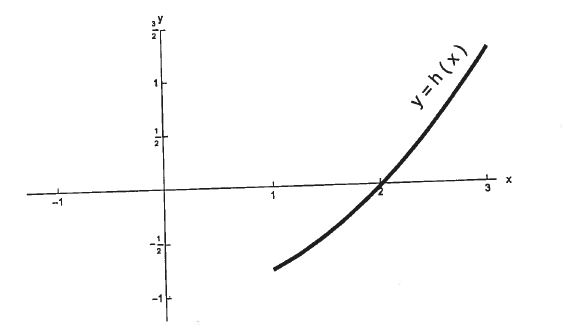
\includegraphics{Figure1}
	\end{image}
	
	\begin{freeResponse}	
	\begin{image}
	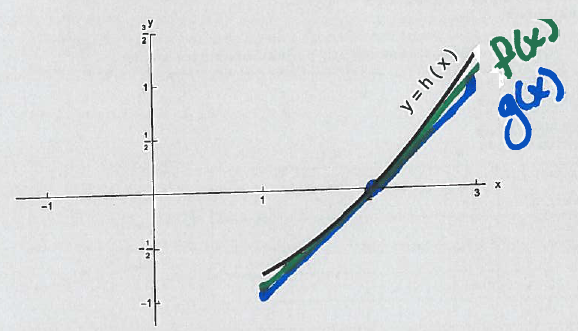
\includegraphics{Figure2}
	\end{image}
	\end{freeResponse}

	\item	Evaluate the limit, or state that it does not exist.  Justify your answer.
		\begin{enumerate}
		\item $lim_{x \to 2} f(x)$
			\begin{freeResponse}
		$g$ and $h$ are both continuous function since they are both polynomials so we have:
		\[
		\lim_{x \to 2} g(x)=g(2)=0
		\]
		\[
		\lim_{x \to 2} h(x)=h(2)=0
		\]
		$g$ and $h$ are both continuous function since they are both polynomials.

		We have $g(x) \le f(x) \le h(x)$ so by the squeeze theorem, $\lim_{x \to 2} f(x)=0$
			\end{freeResponse}

		\item $\lim_{x \to 2} \frac{f(x)+2}{x-1}$
			\begin{freeResponse}
			\[
			\lim_{x \to 2}\frac{f(x)+2}{x-1}=\frac{\lim_{x \to 2}(f(x)+2)}{\lim_{x \to 2}(x-1)}\\
			= \frac{0+2}{0-1}\\
			= \frac{2}{-1}\\
			= -2
			\]
			\end{freeResponse}
		\item $\lim_{x \to 2} g(1+e^{f(x)})$
			\begin{freeResponse}
			\[
			\lim_{x \to 2} g(1+e^{f(x)})= g (\lim_{x \to 2} (1+e^{f(x)}))
			=g (1+e^{(\lim_{x \to 2}f(x))})
			=g(1+e^0)=g(2)=0
			\]
			\end{freeResponse}

		\end{enumerate}
	\item State the form of the limit, evaluate the limit, or state that it does not exist.  Justify your answer.
		\begin{enumerate}
		
		\item $\lim_{x \to 2^-}\frac{1}{f(x)}$
		\begin{freeResponse}
		Form: $\frac{\text{number}}{0}$ \\
		In the fraction: the numerator $1 \to1$ while the denominator $f(x) \to 0^-$ \\			
		Therefore: $\lim_{x \to 2^-}\frac{1}{f(x)}=\infty$
	 
		\end{freeResponse}		

		\item $\lim_{x \to 2}\frac{\frac{x^2-4}{4}}{x-2}$

		\begin{freeResponse}
		Form: $\frac{\text{0}}{0}$ \\
		\begin{align*}
		\lim_{x \to 2}\frac{\frac{x^2-4}{4}}{x-2}&=\lim_{x \to 2}\frac{(x-2)(x+2)}{4}\cdot \frac{1}{x-2}\\
		&= \lim_{x \to 2^+} \frac{x+2}{4}\\
		&= \frac{4}{4}\\
		&= 1
		\end{align*}
		\end{freeResponse}	

		\item $\lim_{x \to 2^+}\frac{h(x)}{g(x)}$

		\begin{freeResponse}
		Form: $\frac{\text{0}}{0}$ \\
		This problem requires us to use the Squeeze Theorem.  We have: \\ 
		\begin{center}
		$g(x) \le f(x) \le h(x)$ \\

		We can divide each side by $g(x)$ since we are concerned with values close to $2$ but not equal to $2$. $\frac{g(x)}{g(x)} \le \frac{f(x)}{g(x)} \le \frac{h(x)}{g(x)}$\\
		$\frac{g(x)}{g(x)}=1$ since $g(x)>0$ when $x>2$\\
		$1 \le \frac{f(x)}{g(x)} \le \frac{h(x)}{g(x)}$\\
		By part ii, we know $\lim_{x \to 2}\frac{h(x)}{g(x)}=1$\\
		$1 \le \frac{f(x)}{g(x)} \le 1$\\
		So by the Squeeze Theorem, $\lim_{x \to 2^+}\frac{h(x)}{g(x)}=1$
			\end{center}
		\end{freeResponse}	

		\end{enumerate}
	
	\end{enumerate}

	
\end{problem}



								
				
				
	














\end{document} 


















